\documentclass[11pt,a4paper]{article}
\usepackage[margin=2.4cm]{geometry}
\usepackage{graphicx,booktabs,amsmath,xcolor,microtype}
\usepackage[colorlinks,linkcolor=blue!55!black,urlcolor=blue!55!black]{hyperref}
\usepackage{caption}
\captionsetup{font=small,labelfont=bf}
\graphicspath{{figures/}}

\newcommand{\tf}{$t_{\mathrm{flash}}$}
\newcommand{\us}{\,$\mu$s}

\title{\textbf{Revising the n\_TOF PSA configuration for the X17 EAR2 campaign}\\
\large What the original production reconstruction gets wrong, and what the
revision measures instead}
\author{X17 / DREAM group}
\date{2026-07-28 \quad run 224572}

\begin{document}
\maketitle

\begin{abstract}
\noindent
The official Pulse Shape Analysis configuration for the 2026 X17 EAR2 campaign
mis-identifies the $\gamma$-flash on the plastic scintillators in
\textbf{37--85\,\% of bunches}, and times the flash on the SiPM walls from the
transient of their own protection gate rather than from the flash itself. Since
every hit's physics time is $\mathrm{tof}-t_{\mathrm{flash}}$, the first defect
shifts whole sets of hits by up to 11.6\us, and the second puts a fixed
$\sim$350\,ns offset between detectors that should agree. Together they made a
hardware wall\,$\wedge$\,plastic coincidence look as though the plastic fired
only half the time.

Both are configuration faults, not detector faults: the raw waveforms contain
the flash, unmissably, in every bunch. This note documents the revision, the
measurements behind each change, and what it costs. On the reference run the
flash mis-identification goes to \textbf{0.0\,\% on 12 of 13 trees}, the
per-arm coincidence offsets go from $-362/{+}20/{-}333/{-}336$\,ns to
$+1.5/{+}2.0/{+}1.0/{-}2.0$\,ns, and our DREAM coincidence matcher improves
from 93.7\,\% to \textbf{96.4\,\%} efficient --- the latter measured with our
offline repair switched off, so it tests the processing alone.
\end{abstract}

\section{Why this was worth chasing}

The X17 measurement pairs the n\_TOF scintillator array with the DREAM
detector. Its trigger is a hardware AND of a SiPM wall and a plastic
scintillator in the same arm, so every triggered event must have a plastic
partner. In the official reconstruction only about half of them did.

The explanation is not in the detectors. It is that
$t_{\mathrm{since\,flash}} = \mathrm{tof}-t_{\mathrm{flash}}$ is only as good
as the PSA's flash identification, and on the plastics that identification
fails in most bunches.

\section{Defect 1: the plastic flash is mis-identified}

The plastic row of the UserInput sets \texttt{G-FLASH THRESHOLD = 50.} with no
lower time limit. The plastic flash saturates the digitiser --- it drives the
signal from a baseline near 30\,800 past zero --- so 50 channels is about
0.2\,\% of the feature it is meant to find. Whatever noise excursion happens
first in the 11.6\us\ before the flash wins instead.

\begin{figure}[htbp]\centering
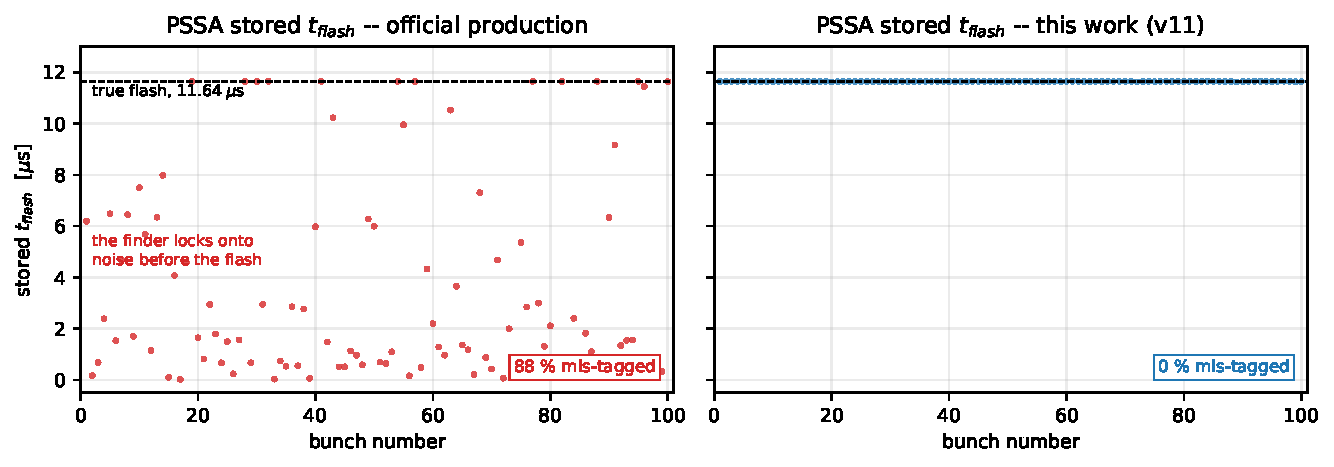
\includegraphics[width=\textwidth]{fig1_flash_id.pdf}
\caption{Stored \tf\ for each bunch of tree PSSA. \emph{Left}: the official
production. The true flash is the dashed line at 11.64\us; most bunches are
tagged somewhere in the noise before it, some by more than 11\us. \emph{Right}:
the same bunches after the revision. Each mis-tagged bunch shifts \emph{all} of
its hits by the tagging error.}
\label{fig:flashid}
\end{figure}

\begin{figure}[htbp]\centering
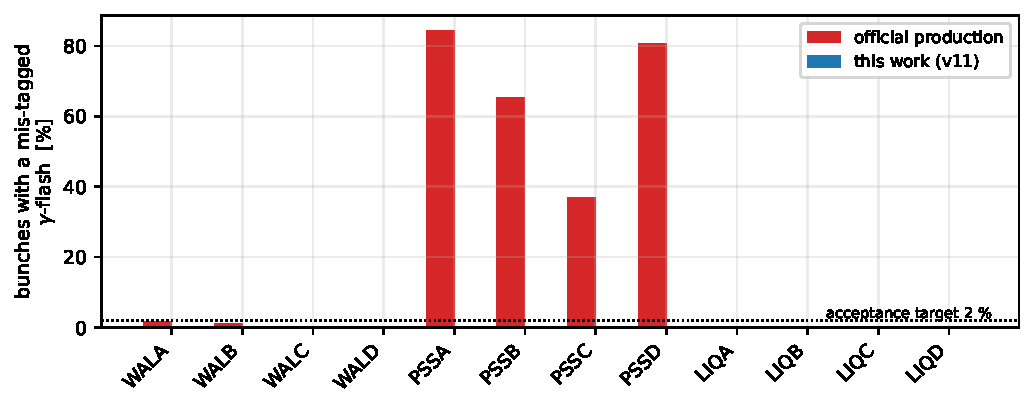
\includegraphics[width=0.86\textwidth]{fig2_bad_fraction.pdf}
\caption{Fraction of bunches whose stored \tf\ is more than 150\,ns from that
tree's own per-run mode, over 421 bunches. The liquids and the pickup are
already clean, which is what shows the plastics' failure is configuration and
not beam.}
\label{fig:badfrac}
\end{figure}

The fix is to give the finder a threshold matched to the feature and a lower
time limit: \texttt{G-FLASH THRESHOLD = 2000/1e4}. The flash sits at 11.63\us\
in every bunch by hardware, so refusing to look before 10\us\ removes the
entire failure mode. The plateau is wide --- 500, 2000 and 5000 give identical
results on 851 channel--bunch combinations --- so the choice is not delicate.

\section{Defect 2: the walls time their own protection gate}

The SiPM wall signal is blanked by a $\sim$1\us\ protection gate around the
flash. The walls therefore never see the flash directly. What the digitiser
records, in order, is: the gate \emph{closing} at 11.24\us; a clamped copy of
the real flash leaking through the closed gate at 11.60\us; and the gate
\emph{opening} at 12.3\us\ with a rail-to-rail transient whose baseline takes
tens of microseconds to recover.

\begin{figure}[htbp]\centering
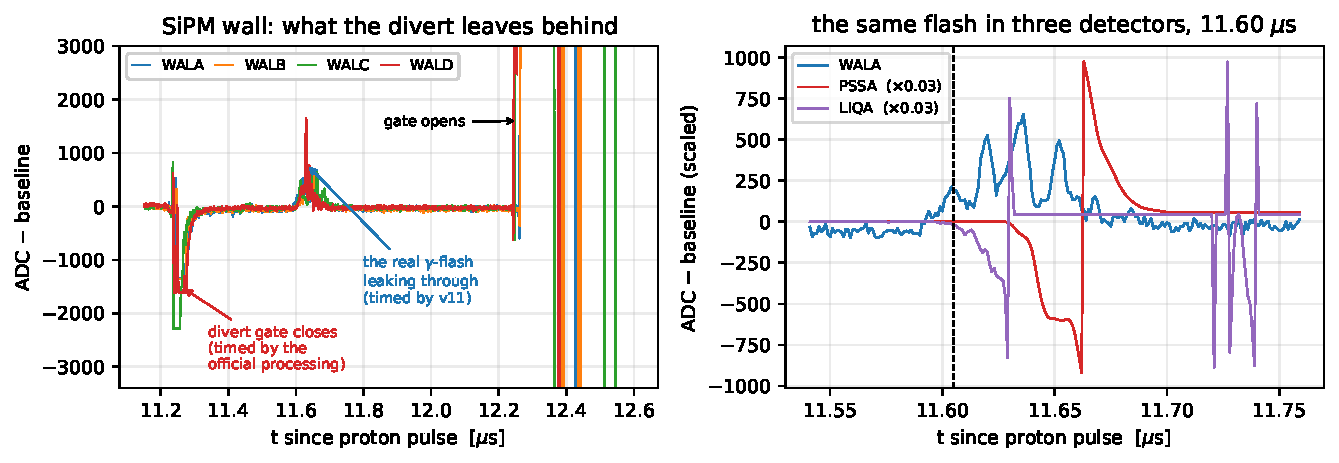
\includegraphics[width=\textwidth]{fig3_divert.pdf}
\caption{Raw stream1 waveforms, bunch 161. \emph{Left}: one channel of each
wall through the gate window. \emph{Right}: the leak seen by the wall next to
the same flash in a plastic and a liquid, neither of which is gated (scaled by
0.03). All three rise at 11.60\us: the wall feature really is the flash.}
\label{fig:divert}
\end{figure}

With \texttt{G-FLASH THRESHOLD = 500.} and no time limit, which of the first
two features wins is decided by their relative amplitude --- and WALB's gate
transient is the weakest of the four walls, so WALB usually lands on the flash
while WALA/C/D land on the gate. \textbf{That bistability is the origin of the
$\sim$350\,ns cross-detector offset}, and it is why arm B looked innocent while
the other three did not.

\begin{figure}[htbp]\centering
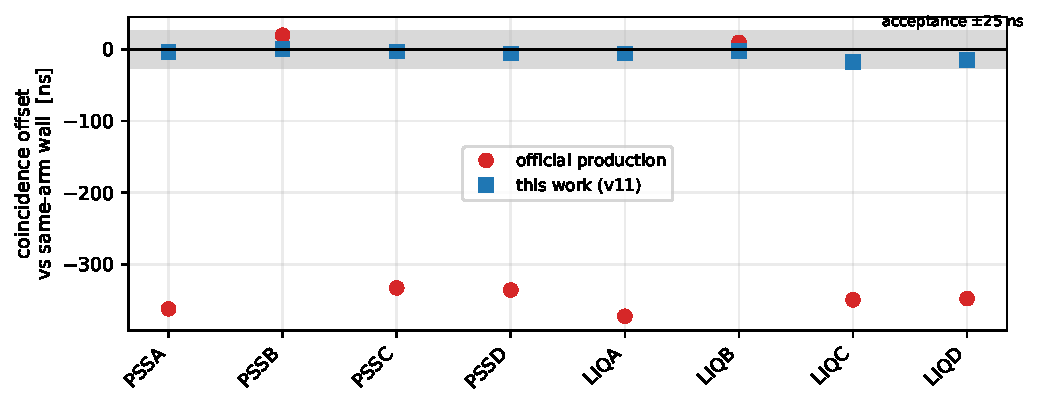
\includegraphics[width=0.86\textwidth]{fig4_coincidence.pdf}
\caption{Position of the prompt coincidence peak between a large hit in each
plastic or liquid and a hit in the same arm's wall. A genuine coincidence
should sit at zero. In the official processing three arms out of four are
displaced by the gate's lead time.}
\label{fig:coinc}
\end{figure}

The fix is a lower time limit placed between the two features:
\texttt{G-FLASH THRESHOLD = 250/11400}. The threshold must stay at or below
400: at 600 the weakest channels miss the leak entirely and fall through to the
gate-opening transient, at which point the spread explodes from $\sim$30\,ns to
$\sim$660\,ns.

\paragraph{What the divert costs regardless.} After the gate reopens the wall
baseline is $+21\,500$ channels at 13\us\ and still $+400$ at 30\us. Wall hits
are unusable from about 11.6 to 13--15\us\ and degraded to $\sim$40\us ---
$E_n$ above roughly 1\,keV at the 19.5\,m flight path. This is a property of
the hardware, not of the configuration, but it belongs in any flux or $E_n$
analysis.

\section{Elimination windows that removed real pulses}

\begin{table}[htbp]\centering\small
\caption{Area/amplitude of isolated late-time pulses, measured directly from
the raw waveforms, against the shipped elimination window.}
\begin{tabular}{lccc}
\toprule
family & measured p1 \dots p99 & shipped cut & fraction removed \\
\midrule
WAL & 42 \dots 110 & 10 \dots 200 & 0\,\% \\
PSS & 1.3 \dots 29 & 2 \dots 20 & $\sim$25\,\% \\
LIQ & 1.7 \dots 14 & 2 \dots 10 & $\sim$19\,\% \\
\bottomrule
\end{tabular}
\label{tab:areaamp}
\end{table}

The wall cut sits a factor two above the largest value the walls ever produce,
which is what a safe elimination window looks like; the plastic and liquid cuts
sit inside the bulk of their own distributions (Fig.~\ref{fig:areaamp}). Both
were widened to $1\dots60$. The PSA guide is explicit that elimination should
be loose and that final rejection belongs in the offline analysis.

\begin{figure}[htbp]\centering
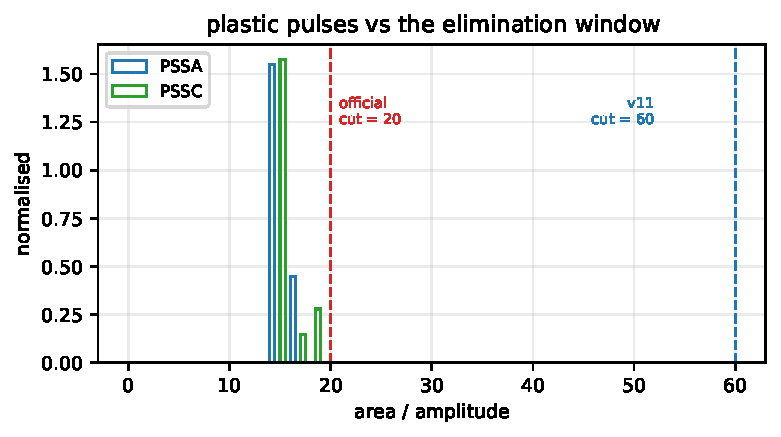
\includegraphics[width=0.62\textwidth]{fig6_areaamp.pdf}
\caption{Area/amplitude of plastic pulses in the revised processing, with the
old and new upper cuts marked. Everything to the right of the red line was
being discarded.}
\label{fig:areaamp}
\end{figure}

\section{Pulse shapes}

\subsection{The walls: the shipped templates are too short}

Each shipped wall template is a \emph{single raw pulse}, 314\,ns long. The wall
pulse is still at 4--6\,\% of its peak 200\,ns after the maximum and 0.5\,\% at
500\,ns, so the template ends inside the tail (Fig.~\ref{fig:templates}). Every
fitted amplitude then mis-accounts that tail, and the pileup deconvolution is
working with a truncated kernel.

\begin{figure}[htbp]\centering
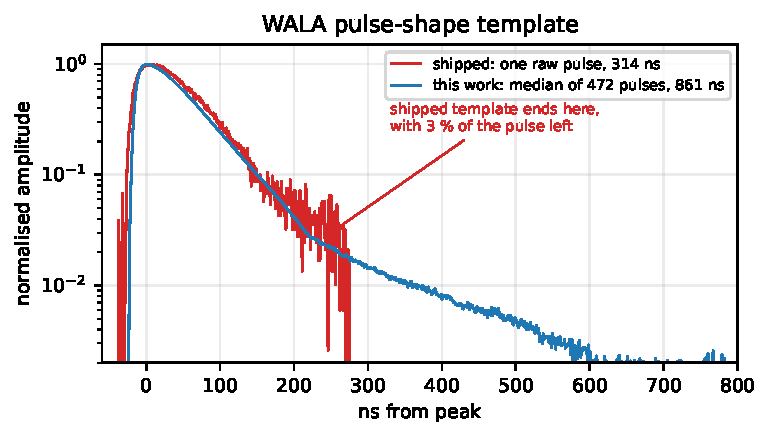
\includegraphics[width=0.62\textwidth]{fig5_templates.pdf}
\caption{WALA pulse-shape template, normalised, logarithmic. The replacement is
the median of 472 clean isolated pulses and runs to 861\,ns.}
\label{fig:templates}
\end{figure}

\begin{table}[htbp]\centering\small
\caption{Median fit $\chi^2$ per wall, shipped vs measured templates.}
\begin{tabular}{lcccc}
\toprule
 & WALA & WALB & WALC & WALD \\
\midrule
shipped (single pulse, 314\,ns) & 0.896 & 1.227 & 1.133 & 1.184 \\
measured (median, 720--861\,ns) & \textbf{0.851} & \textbf{1.002} & \textbf{1.002} & \textbf{1.062} \\
\bottomrule
\end{tabular}
\end{table}

\subsection{The plastics: fitting enabled, and it was the largest single gain}

The plastics used \texttt{AMPLITUDE OPTION = 1} --- a parabolic fit to the top,
no deconvolution at all --- while being the highest-rate tree in the file.
Switching to shape fitting with measured 101\,ns templates produced the biggest
downstream improvement of any change, and by an instructive route: it yields
\emph{fewer} plastic hits (0.72--0.99 of the previous count at every amplitude
cut) but \emph{better-timed} ones, merging pileup fragments back into a single
correctly-timed pulse. The number of valid wall\,$\wedge$\,plastic candidates
rises even as the number of plastic hits falls.

\subsection{The liquids: three attempts, all worse}

We tried replacing the liquid templates three times --- 551\,ns averages,
81\,ns averages, per-detector rather than shared --- and every attempt was
worse, with $\chi^2$ more than doubling and amplitudes falling $\sim$30\,\%.
The shipped liquid pair spans FWHM 1\,ns and 7\,ns, a near-delta plus a normal
pulse, and we suspect that spread does real work that a set of similar averaged
shapes cannot reproduce. \textbf{The shipped liquid templates are kept.} We
record the failure because it is the kind of change that looks obviously good
and is not.

\section{What the revision achieves, and what it costs}

\begin{figure}[htbp]\centering
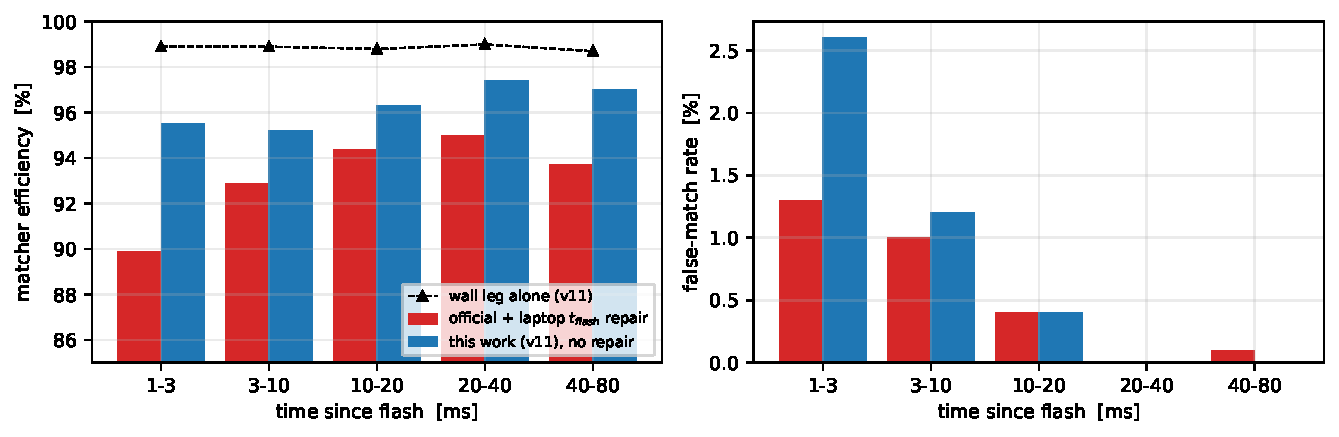
\includegraphics[width=\textwidth]{fig7_efficiency.pdf}
\caption{DREAM coincidence matcher, thresholded wall\,$\wedge$\,plastic
singles. \emph{Left}: efficiency per time-since-flash bin; the triangles are
the wall leg alone, which shows the plastic leg is what limits the AND.
\emph{Right}: the false-match rate, measured with a $+100\,\mu$s time-shifted
control. The official column already includes our offline \tf\ repair --- with
the raw official file the matcher is 12.7\,\% efficient and unusable.}
\label{fig:eff}
\end{figure}

\begin{table}[htbp]\centering\small
\caption{Summary on run 224572, DREAM run\_79/stat090\_0000. The revised column
is measured with our offline \tf\ repair \emph{disabled}.}
\begin{tabular}{lcc}
\toprule
 & official production & this revision \\
\midrule
flash mis-identification & PSS 37--85\,\% & 0.0\,\% on 12 of 13 trees \\
per-arm coincidence offset & $-362/{+}20/{-}333/{-}336$\,ns & $+1.5/{+}2.0/{+}1.0/{-}2.0$\,ns \\
matcher efficiency & 93.7\,\% \emph{(needs our repair)} & \textbf{96.4\,\%} \\
matcher false rate & 0.5\,\% & 0.6\,\% \\
\quad in the 1--3\,ms bin & 89.9\,\% / 1.3\,\% & \textbf{95.5\,\%} / 2.6\,\% \\
\midrule
wall timing, top$\leftrightarrow$bottom $\sigma$ & \multicolumn{2}{c}{6.65\,ns $\rightarrow$ 6.65\,ns} \\
wall$\leftrightarrow$plastic coincidence $\sigma$ & \multicolumn{2}{c}{6.46\,ns $\rightarrow$ 6.41\,ns} \\
MIP peak width (FWHM/peak) & \multicolumn{2}{c}{1.22 $\rightarrow$ 1.22} \\
timing walk over amplitude & \multicolumn{2}{c}{1.38\,ns $\rightarrow$ 1.48\,ns} \\
\bottomrule
\end{tabular}
\end{table}

The lower half of that table is the guard: it would be easy to gain hits by
reconstructing them worse, so timing resolution, amplitude linearity and MIP
width were tracked alongside efficiency. All are unchanged within a few
percent.

\paragraph{The cost, stated plainly.} The false-match rate in the 1--3\,ms bin
roughly doubles, from 1.3\,\% to 2.6\,\%. That is the direct consequence of
recovering the plastic hits: the candidate rate rises from $\sim$935 to
$\sim$1042 per bunch. For this analysis it is a good trade, because efficiency
in the same bin rises by 5.6 points and accidentals can be subtracted offline
with a time-shifted control. An analysis that needs early-time purity instead
can trade it back by tightening \texttt{AREA/AMP HIGH} towards 20.

\paragraph{Where the limit now is.} The wall leg alone reaches 98.9\,\% and is
flat in time; the AND reaches 96.4\,\%. The plastic leg therefore still costs
2.5\,\% overall and 3.4--3.7\,\% at early times. We established that this is
\emph{not} a pulse-recognition problem: three further variants with materially
different plastic reconstructions --- $\pm$40\,\% in amplitude, $\pm$30\,\% in
hit count --- all return exactly 96.4\,\%, because above $\sim$2000\,ADC they
agree to better than 1\,\% and the hardware discriminator never sees anything
below that. Further gains are analysis-side: the per-arm discriminator
threshold model, the channel selection, dead time, or real detector
inefficiency.

\begin{figure}[htbp]\centering
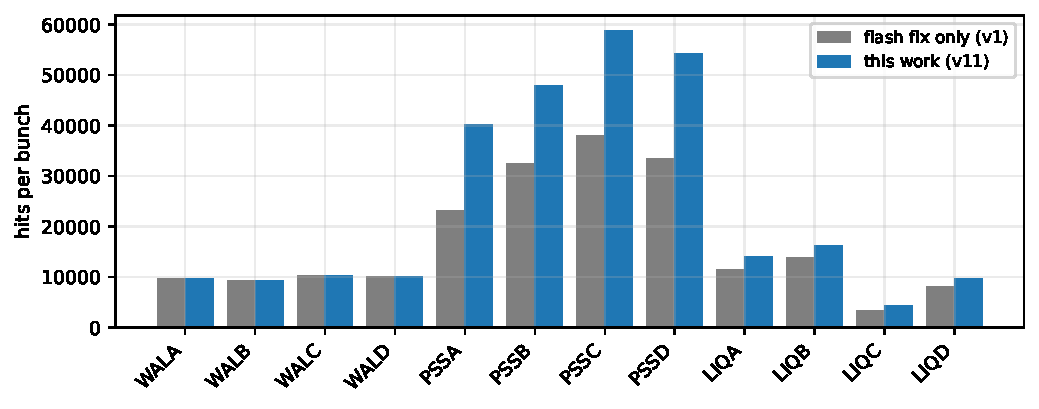
\includegraphics[width=0.86\textwidth]{fig8_hits.pdf}
\caption{Hits per bunch per tree, flash fix alone versus the full revision. The
walls are unchanged by construction --- their elimination windows were already
safe --- which is the control that the change did what it was meant to and
nothing else.}
\label{fig:hits}
\end{figure}

\section{Reproducing this}

All tooling is in the group repository under \texttt{ntof\_processing/}:
\texttt{grade\_candidate.py} (flash identification, coincidence offsets, hit
counts), \texttt{compare\_fits.py} (fit $\chi^2$),
\texttt{quality\_metrics.py} (timing resolution, amplitude linearity, MIP
width, timing walk --- all accidental-subtracted),
\texttt{dream\_regression.py} (the matcher), \texttt{make\_variants.py}
(generates a UserInput as a base plus named column edits),
\texttt{flash\_finder\_emulator.py} (pre-validates G-FLASH parameters on raw
waveforms without a processing round-trip), and
\texttt{make\_pulse\_shapes.py} (builds the templates). The numbers quoted here
are in \texttt{report/results.json} with the tool that produced each one.

\paragraph{Two traps worth passing on.} Coincidence widths must be
accidental-subtracted: at these rates the nearest-hit-in-window distribution is
dominated by chance, and without an off-time sideband subtracted the
wall$\leftrightarrow$plastic width reads 38.8\,ns instead of 6.4\,ns. And the
merge step of \texttt{RunProcessing.sh} failed on every EAR2 run we tried, with
\texttt{max total download bytes exceeded (max=1024 MB)} --- the per-file
processing always succeeded, so we read the partials in \texttt{completed/}
directly.

\end{document}
